\subsection{Prostate Anatomy}
The prostate gland sits caudal to the urinary bladder and surrounds the urethra.
Its superior borders include the bladder and seminal vesicles, and the
urogenital diaphragm delineates its inferior boundary. The gland is bordered
anteriorly by the pubic symphysis and posteriorly by the rectum.  The prostate
is separated from the rectum by a 2--3 mm fascial layer,~\cite{Jung2012} and it
can be easily palpated on rectal examination. 

The prostate gland can be divided from superior-to-inferior into the base,
mid-gland and apex. The urethra enters the prostate proximally at the base and
extends to the mid-gland, at which point the ejaculatory ducts open into the
urethra at the verumontanum.~\cite{Jung2012} The urethra then continues past
the apex and travels through the penis. The prostate can be divided into
glandular and non-glandular components.  The glandular components include the
transitional zone (TZ), central zone (CZ) and peripheral zone (PZ)
(Figure~\ref{fig:mcneal_anatomy}). In the healthy prostate, each zone contains
approximately 5\%, 20\% and 70--80\% of glandular tissue,
respectively~\cite{Bonekamp2011}, but these ratios can change significantly in
the presence of benign prostatic hyperplasia (BPH). The non-glandular
components include the anterior fibromuscular stroma (AFS) and the urethra.  In
some imaging modalities, the central and transition zones cannot be visualized
as discrete entities, and they are collectively identified as the central gland
(CG).  The CG was one of the prostate structures manually segmented in MR and
ARFI images in this study.

\begin{figure}
\centering
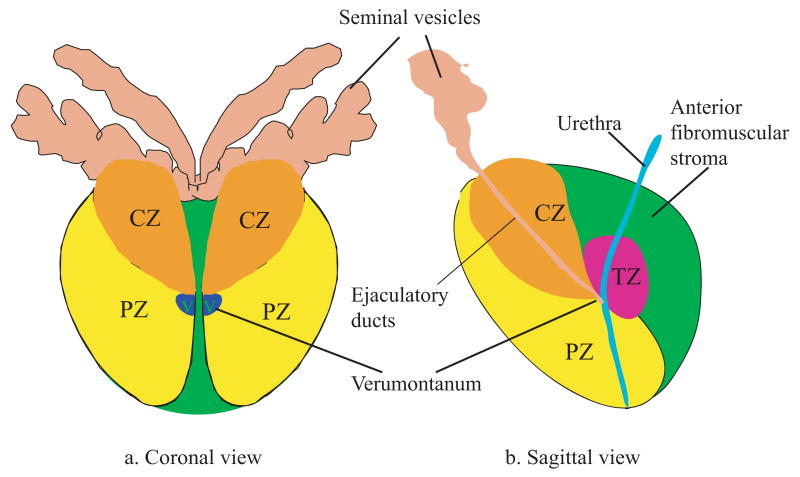
\includegraphics[width=0.75\linewidth]{figs/Mcneal_Zonal_Anatomy.jpg}
\caption{\textbf{Diagrams of McNeal’s zonal anatomy of the human
    prostate.~\cite{mcneal_path} It divides a human prostate into one
    nonglandular zone (the anterior fibromuscular stroma) and three glandular
    zones: central zone, peripheral zone and transition zone, denoted by CZ, PZ
    and TZ, respectively. (a) Coronal section of the prostate. V represents the
    verumontanum. (b) Sagittal section of the prostate. In the top part of the
    diagram, the seminar vesicles and ductus deferens enter the central zone
    and connect to the ejaculatory ducts, which merge with the urethra at the
    verumontanum. (Figure reprinted with permission.~\cite{Zhai2010a})}}
\label{fig:mcneal_anatomy} 
\end{figure}


An outer band of fibromuscular tissue surrounds the anterior aspect of the
prostate.~\cite{Bonekamp2011} This boundary is important when assessing the
extraprostatic extension of cancer as tumor can spread by disrupting this
tissue. Two neurovascular bundles course posterior and lateral to the prostate,
which can also be invaded by malignant cells.  The prostate capsule is another
structure that was manually segmented in both MR and ultrasound images in this
study, and its overall extent was used to delineate the total prostate gland.
